\section{natural alternating diagram}

Suppose we have a Riemann sphere $C$ with two punctures at $0$ and $\infty$. Topologically, $C$ is homeomorphic to the boundaryless cylinder(figure below)
\begin{figure}[H] % Optional: [h] means here, [t] for top, [b] for bottom, [p] for page of floats
    \centering
    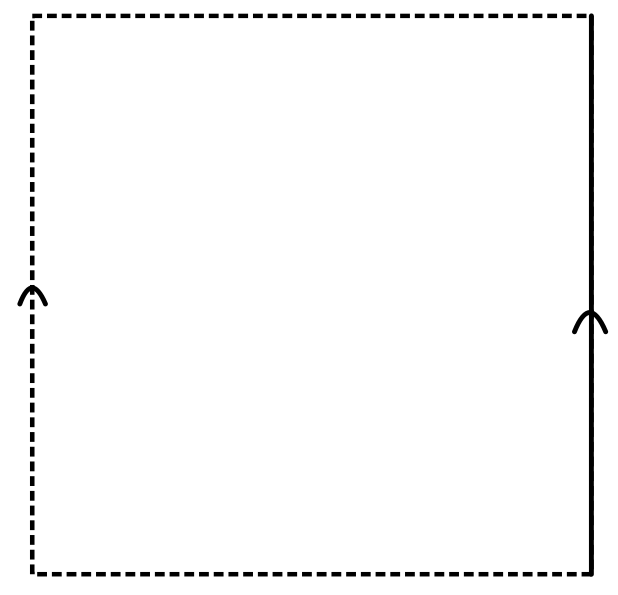
\includegraphics[scale = 0.95]{diagrams/natural_alternating_diagrams/1.png} % Adjust the width as needed
    \caption{Your caption here}
    \label{fig:your-label}
\end{figure}


Suppose we have a braid word $\omega$, then we can draw the associated braid diagram($i_1,\cdots, i_{n -1}: [0,1]\rightarrow [0,1] \times (0,1)$) on $[0,1] \times(0,1)$ and its cylindrical closure on $S^1 \times (0,1)$ as shown below.
\begin{figure}[H] % Optional: [h] means here, [t] for top, [b] for bottom, [p] for page of floats
    \centering
    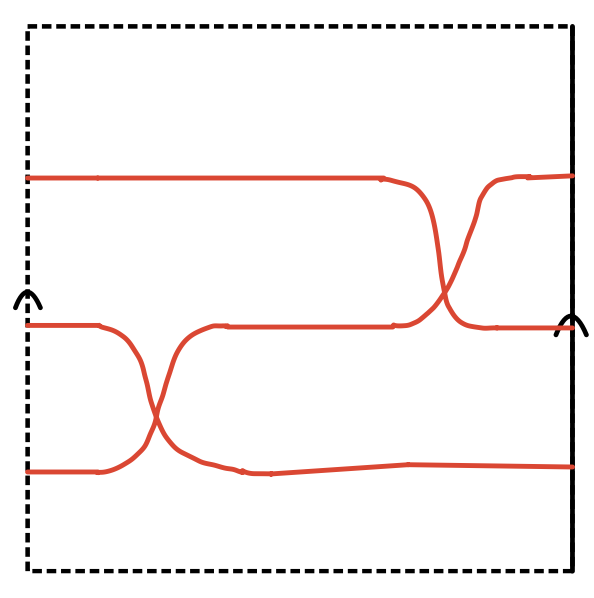
\includegraphics[scale = 0.95]{diagrams/natural_alternating_diagrams/2.png} % Adjust the width as needed
    \caption{Your caption here}
    \label{fig:your-label}
\end{figure}


We will specify co-orientations of $i_1, \cdots, i_{n-1}$ so that we can think of the cylindrical closure of the braid word as the the front projection Legendrian knot living inside the co-circle bundle of the cylinder.

we define the co-orientation at $i_k(t_0)$ to be $\xi = adx + bdy$ so that $\xi$ vanishes at $\frac{di_k}{dt}(t_0)$,$||(a,b)||= 1$, and $b>0$. This can be visually represented as hairs pointing upward($b>0$).

\begin{figure}[H] % Optional: [h] means here, [t] for top, [b] for bottom, [p] for page of floats
    \centering
    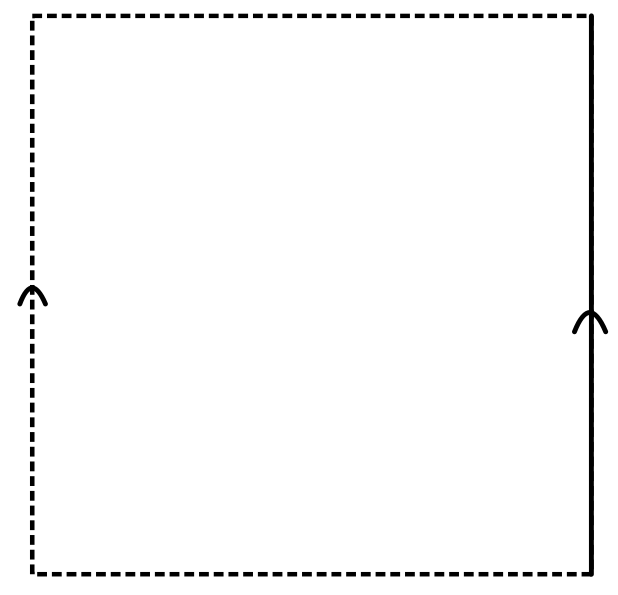
\includegraphics[scale = 0.95]{diagrams/natural_alternating_diagrams/3.png} % Adjust the width as needed
    \caption{Your caption here}
    \label{fig:your-label}
\end{figure}

There are two different ways of embedding this cylindrical closure into $C$. We can embed this cylindrical closure onto the hemisphere containing $0$($\infty$ resp.) in such a way that the embedding extends
\begin{enumerate}[label = (roman*)]
\item to $S^1 \times \{ 0 \}$) as an isomophism onto the equator of $C$
\item to  $S^1 \times \{ 1 \}$ as a constant map to $0$($\infty$ resp.)
\end{enumerate}

\begin{figure}[H] % Optional: [h] means here, [t] for top, [b] for bottom, [p] for page of floats
    \centering
    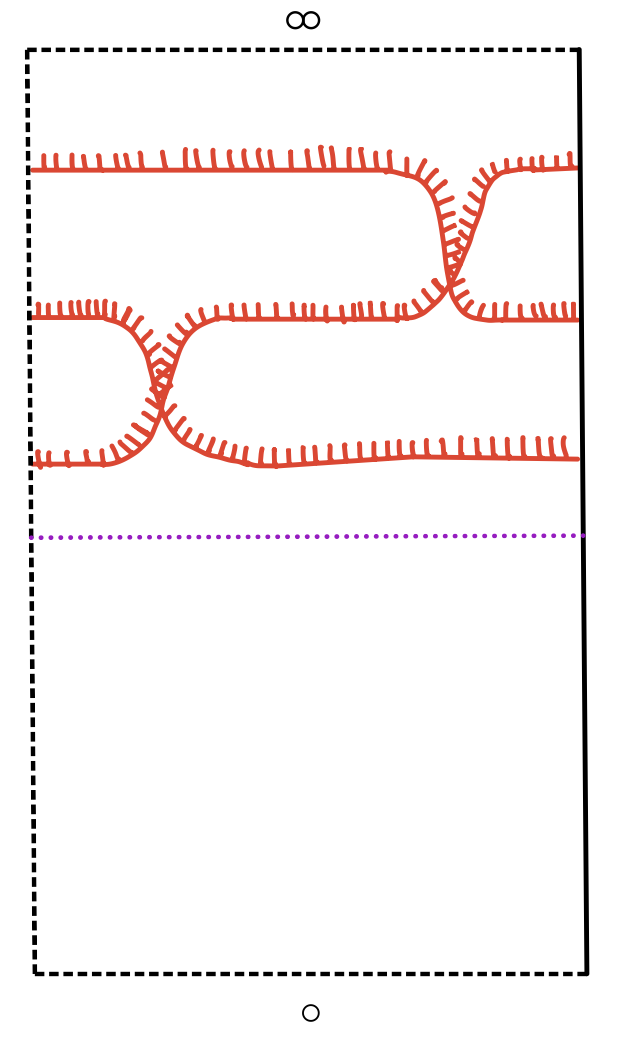
\includegraphics[scale = 0.95]{diagrams/natural_alternating_diagrams/4-1.png} % Adjust the width as needed
    \caption{embedding of the cylindrical closure onto the hemisphere containing $\infty$}
    \label{fig:your-label}
\end{figure}

\begin{figure}[H] % Optional: [h] means here, [t] for top, [b] for bottom, [p] for page of floats
    \centering
    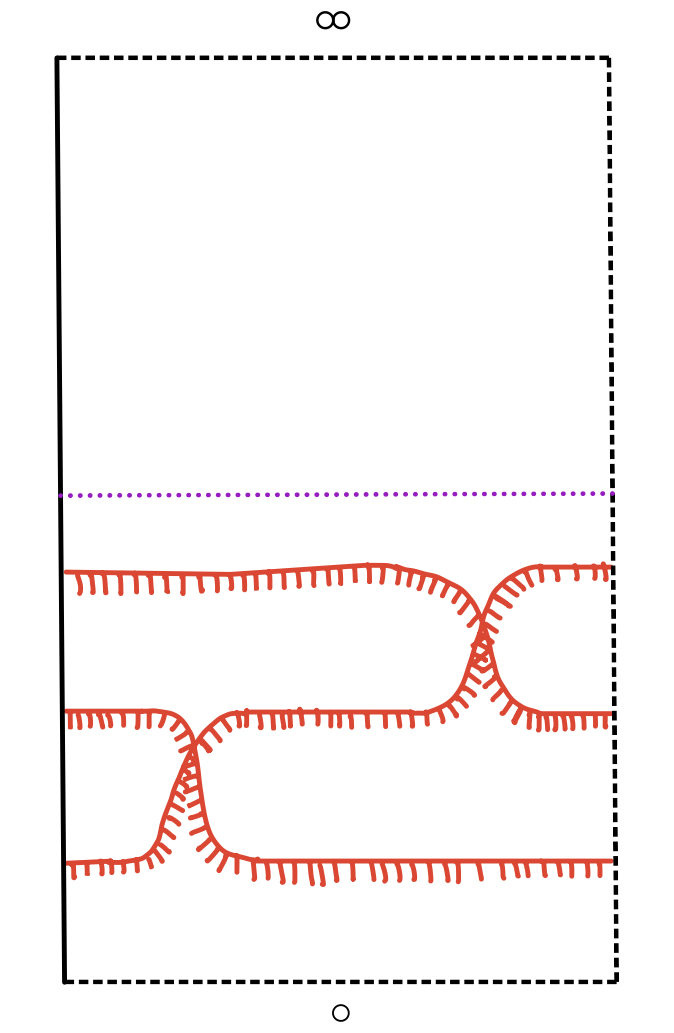
\includegraphics[scale = 0.95]{diagrams/natural_alternating_diagrams/4-2.png} % Adjust the width as needed
    \caption{embedding of the cylindrical closure onto the hemisphere containing $0$}
    \label{fig:your-label}
\end{figure}


Suppose we have a braid word $\omega$ on $n$ strands. 
Consider the following associated object : 
\begin{itemize}
\item $C$ : 
A Riemann sphere with two punctures at $0$ and $\infty$

\item $\iota_0 : (S^1)^n->  C$
the link given by the embedding of the cylindrical closure of the trivial braid word onto the hemisphere containing $0$

\item $\xi_0$ : co-orientation of $\iota_0$

\item $\iota_\infty : (S^1)^m->  C$ (where $m \leq n$)
the link given by the embedding of the cylindrical closure of the braid word $\omega$ onto the hemisphere containing $\infty$

\item $\xi_\infty$ : co-orientation of $\iota_\infty$
\end{itemize}



we will denote the union of 
\begin{itemize}
\item two embeddings $\iota_0$ and $\iota_\infty$ as $\iota$ 
\item $\xi_0$ and $\xi_\infty$ as $\xi$
\end{itemize}

Now fix a braid word $\omega$ and the object $(C,\iota,\xi)$ associated with it. I will define a natural alternating braid diagram $(C,\iota',\xi')$ whose associated Legendrian is Legendrian isotopic to the Legendrian associated with $(C,\iota,\xi)$ by drawing associated diagram on $C$. The proof of it will be the main contents of this section. The isotopy will be only applied to $\iota_0$, so the $\iota_\infty$ will remain fixed i.e. $\iota_\infty = \iota'_\infty$.

First, let's draw $\iota'_\infty$ as in red on $C$ as follows :

\begin{figure}[H] % Optional: [h] means here, [t] for top, [b] for bottom, [p] for page of floats
    \centering
    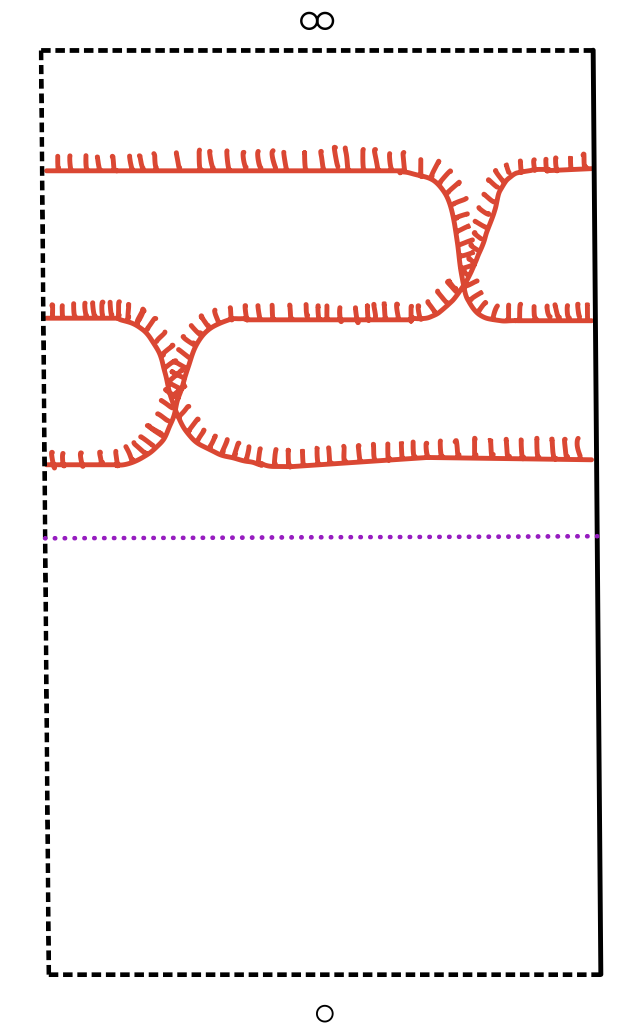
\includegraphics[scale = 0.95]{diagrams/natural_alternating_diagrams/5.png} % Adjust the width as needed
    \caption{Your caption here}
    \label{fig:your-label}
\end{figure}

Now on the above diagram, let's draw ($\iota'_0$) the part that is isotopic to $\iota_0$ in blue. We need some definitions.
Suppose $\omega = s_{1_1},..., s_{i_k}$, then the cylindirical closure can be parsed into concatenation of k mutually disjoint regions where $i^{th}$ region containing a part of the braid diagram corresponding to the generator $s_{i_j}$(figure below). We call the region corresponding to $s_{i_j}$ as the $j^{th}$ generator region(also its image inside under the embedding into $C$).
\begin{figure}[H] % Optional: [h] means here, [t] for top, [b] for bottom, [p] for page of floats
    \centering
    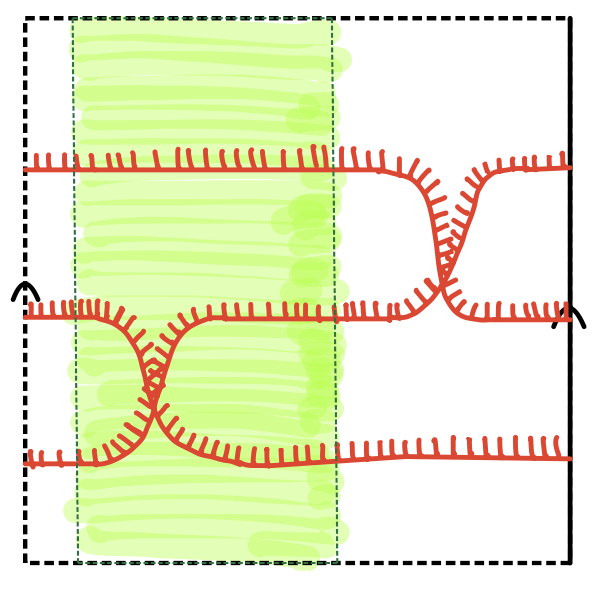
\includegraphics[scale = 0.95]{diagrams/natural_alternating_diagrams/6-1.png} % Adjust the width as needed
    \caption{1st generator region}
    \label{fig:your-label}
\end{figure}

\begin{figure}[H] % Optional: [h] means here, [t] for top, [b] for bottom, [p] for page of floats
    \centering
    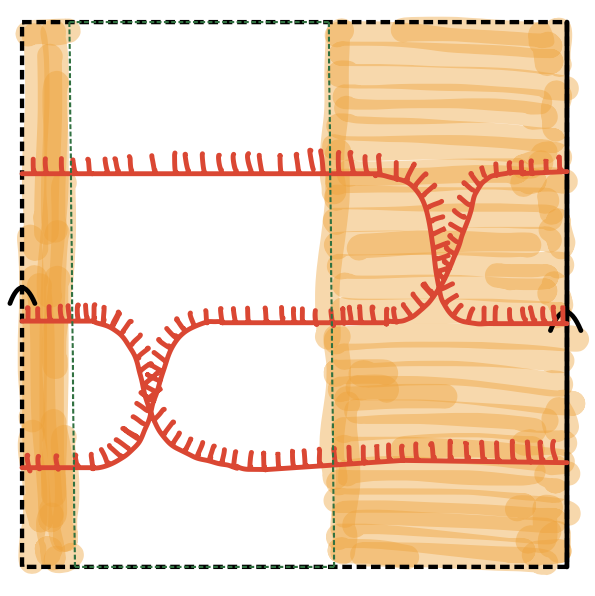
\includegraphics[scale = 0.95]{diagrams/natural_alternating_diagrams/6-2.png} % Adjust the width as needed
    \caption{2nd generator region}
    \label{fig:your-label}
\end{figure}


Suppose we set-theoretically subtract the union of all generator regions from the cylinder, we get $k$ connected components. That is, for each $j = 1,...,k$, we have one component in between $j^{th}$ and $j+1^{th}$(modulo $k$) regions. We call the neighborhood of this component inside the cylinder as  $j^{th}$ inter-generator region(also its image inside the cylinder under the embedding into $C$).
\begin{itemize}
\item inter-generator regions do not contain any crossing
\item inter-generator regions are mutually disjoint
\item $j^{th}$ intergenerator region intersects with $j^{th}$ and $j+1^{th}$(modulo $k$) generator region
\end{itemize}

\begin{figure}[H] % Optional: [h] means here, [t] for top, [b] for bottom, [p] for page of floats
    \centering
    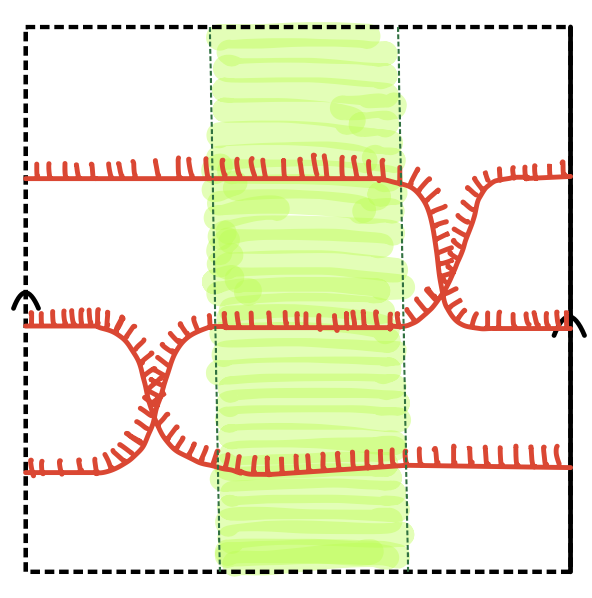
\includegraphics[scale = 0.95]{diagrams/natural_alternating_diagrams/7-1.png} % Adjust the width as needed
    \caption{1st inter-generator region}
    \label{fig:your-label}
\end{figure}

\begin{figure}[H] % Optional: [h] means here, [t] for top, [b] for bottom, [p] for page of floats
    \centering
    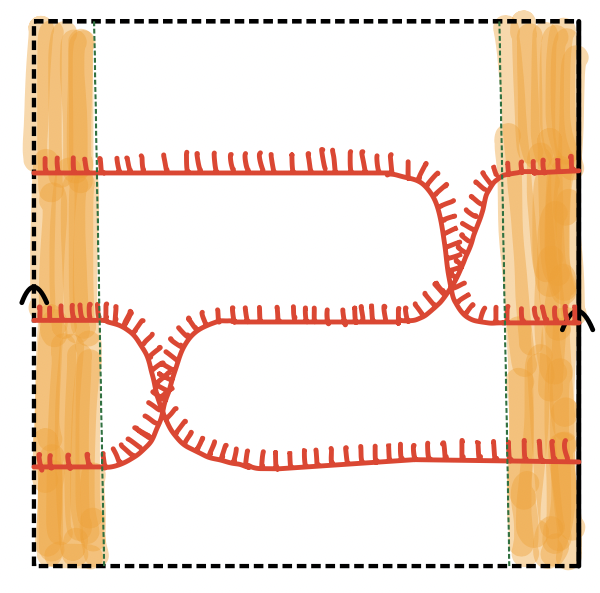
\includegraphics[scale = 0.95]{diagrams/natural_alternating_diagrams/7-2.png} % Adjust the width as needed
    \caption{2nd inter-generator region}
    \label{fig:your-label}
\end{figure}

I will draw $\iota'_0$ for each generator region so that they glue up to the whole $\iota'_0$. 

First, we restrict the diagram to $j^{th}$ generator region, we have the following diagram:

\begin{figure}[H] % Optional: [h] means here, [t] for top, [b] for bottom, [p] for page of floats
    \centering
    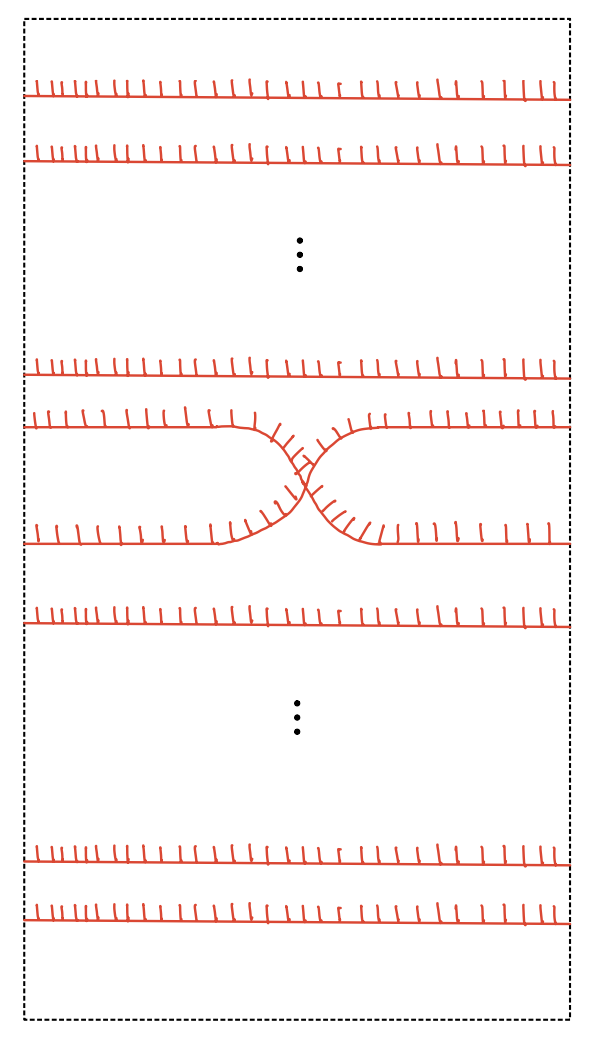
\includegraphics[scale = 0.95]{diagrams/natural_alternating_diagrams/8.png} % Adjust the width as needed
    \caption{Your caption here}
    \label{fig:your-label}
\end{figure}


notation : we number the strands from top to bottom from $1,\cdots,n$ with reference to the left end points.


I will draw $\iota'_0$ as blue strand on it as follows :
\begin{itemize}
\item lth blue strand starts from the midpoint of the starting points of lth and l+1th red strands and ends at the midpoint of the end points of lth and l+1th red strands

\item if $l \neq i_j$ and $i\neq i_j +1$, then along the way the $l^{th}$ blue strand crosses up and down twice

\item if $l = i_j$, $l^{th}$ blue strand crosses $l^{th}$ red strand up in the part before the crossing and then crosses $l+1^{th}$ red strand down in the part after the crossing.

\item if $l = i_j + 1$, $l^{th}$ blue strand crosses $l+1^{th}$ red strand up and down in the part before the crossing and then crosses $l^{th}$ red strand up and down in the part after the crossing.
\end{itemize}

\begin{figure}[H] % Optional: [h] means here, [t] for top, [b] for bottom, [p] for page of floats
    \centering
    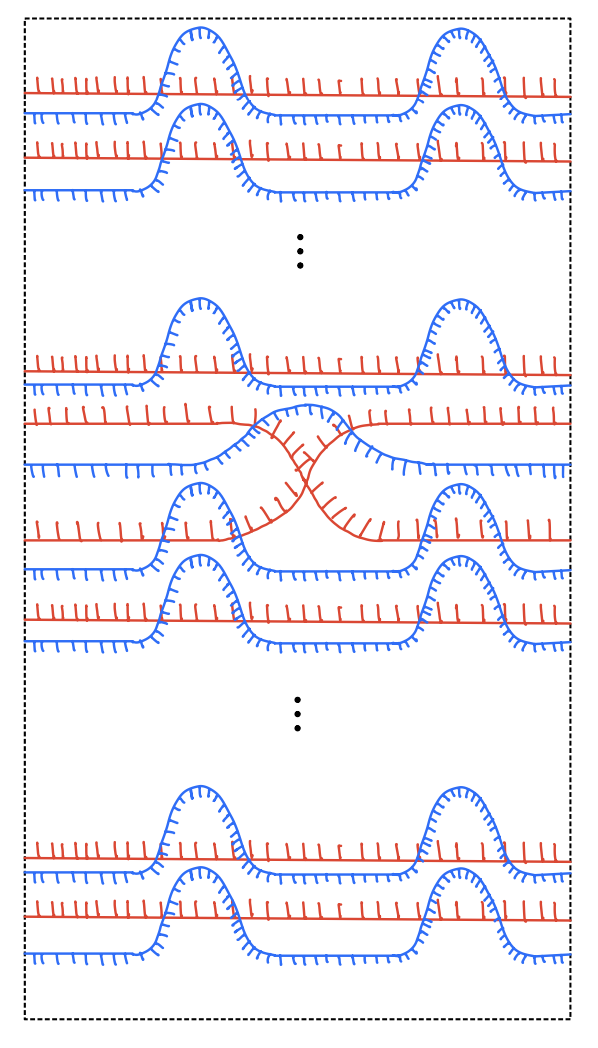
\includegraphics[scale = 0.95]{diagrams/natural_alternating_diagrams/9.png} % Adjust the width as needed
    \caption{Your caption here}
    \label{fig:your-label}
\end{figure}

For the full alternating strand diagram, we take the closure of blue strands from the generator regions so that the end points from the bordering regions coincide.

\begin{figure}[H] % Optional: [h] means here, [t] for top, [b] for bottom, [p] for page of floats
    \centering
    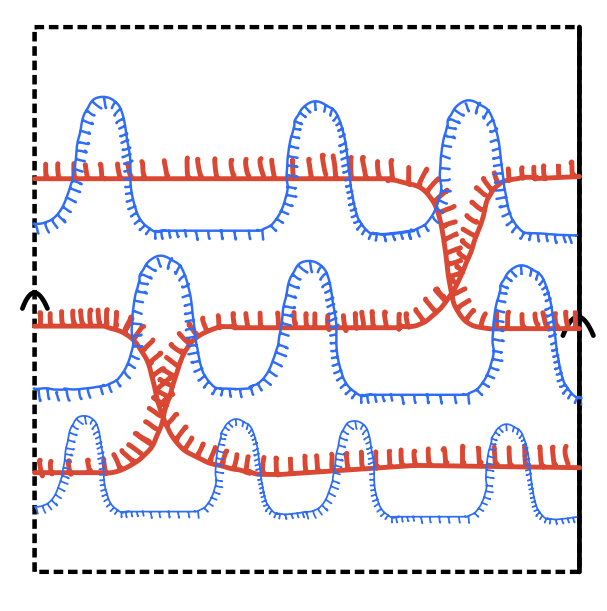
\includegraphics[scale = 0.95]{diagrams/natural_alternating_diagrams/10.png} % Adjust the width as needed
    \caption{Your caption here}
    \label{fig:your-label}
\end{figure}
\begin{theorem}
The above defined strand diagram is alternating
\end{theorem}
(proof) we will denote 
\begin{itemize}
\item the region with all the hairs pointing outward as $\circ$
\item the region with all the hairs pointing inward as $\bigtriangleup$
\item else with $\times$
\end{itemize}

for the generator region we have the following figure :
\begin{figure}[H] % Optional: [h] means here, [t] for top, [b] for bottom, [p] for page of floats
    \centering
    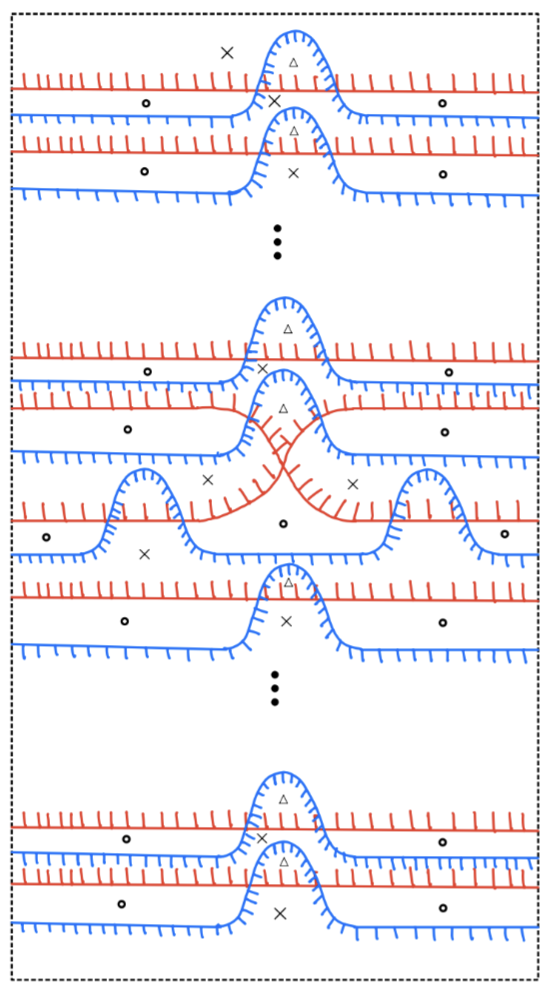
\includegraphics[scale = 0.95]{diagrams/natural_alternating_diagrams/11.png} % Adjust the width as needed
    \caption{Your caption here}
    \label{fig:your-label}
\end{figure}
for the inter-generator region we have the following figure:
\begin{figure}[H] % Optional: [h] means here, [t] for top, [b] for bottom, [p] for page of floats
    \centering
    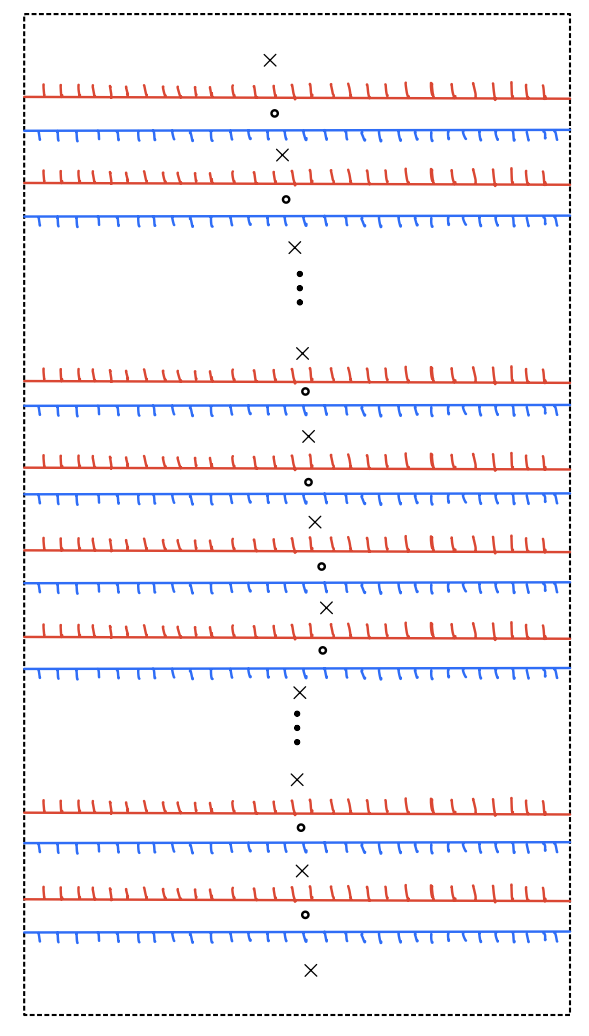
\includegraphics[scale = 0.95]{diagrams/natural_alternating_diagrams/12.png} % Adjust the width as needed
    \caption{Your caption here}
    \label{fig:your-label}
\end{figure}
for each crossing, it satisfy the alternating condition. This diagram is indeed alternating.